\chapter{准备工作}
\section{开箱}
打开包装箱,取出机器人本体、控制箱、电源线、配件包等产品。
\vspace*{-6pt}

\section{安全指南}
\label{sec:安全指南}
在将机器人安装和上电之前,请务必认真仔细阅读此节内容,并严格按照正确的顺序和方式安装和启动机器人。

\subsection{安全警示标志}

\dange{出现此标志时,请特别关注警示说明中可能导致用电危险的情况,如果不注意,可导致人员伤亡、伤害或设备损坏。}

\danger[危险/警告]{出现此标志时,请特别关注警示说明中可能导致人身安全、设备损坏的情况,如果不注意,可导致人员伤亡、伤害或设备严重损坏。}

\info{出现此标志时,请关注在操作过程中需要注意的事项,如果不注意,可能造成错误操作,引起误伤。}

\subsection{安装环境条件}
安装机器人前,应该先检查安装环境条件是否符合要求,以免造成机器人故障或引起误伤。

\begin{itemize}
\item 环境温度:$0\sim 40\,$℃
\item 环境相对湿度:$25\%\sim 85\%$
\item 周围环境:无腐蚀性气体或液体、无油烟或盐雾、无灰尘或金属屑、无放射性材料、无易燃物品、无电磁噪声、无放射性材料,尽量避免阳光直射。
\item 作业空间:必须确保足够安全作业(拖动示教、维修等)的空间。
\item 安装表面:安装机器人时,需选择一个坚固且防震的表面,该表面需要可以承受至少10倍的底座关节完全扭转力(底座关节最大扭矩$40 \Nm$),以及至少5倍的机器人重量(机器人本体自重$9.5 \kg$)。
\end{itemize}

\vfill
\newpage

\info{\begin{itemize}
	\item 使用环境,避免设备进水进尘进油烟等,如有类似场景注意遮蔽设备;
	\item 不可拆解机器,避免造成产品损坏;
	\item 产品拆装过程中,轻拿轻放,防止磕碰、摔落。
\end{itemize}}

% \clearpage

\danger{机器人需要安全地放置在坚固防震表面上,请确保机器人操作不会受到冲击、震动影响,否则机器人安装螺钉松脱可能会造成机器人倾倒,引起误伤或财产损失。}
\danger{请确保安装环境中无易燃气体、易燃粉尘、易燃液体等物质,否则可能造成爆炸或引起火灾。}
\danger{请确保安装环境中无水、腐蚀性气体、金属屑、灰尘等物质,同时确保安装环境温度与湿度在允许范围内,否则可能会造成机器人误动作、故障或漏电。}
\danger{请勿在超过机器人抗电磁干扰、静电放电能力等范围的环境中使用,否则可能造成机器人停机,运行轨迹发生变化,产生不可预估的危险。\footnote{详见\prettyref{app:参照标准}。}}

% \clearpage

\subsection{安装注意事项}
控制箱应水平放置,两侧进出风口应至少保留$5 \cm$空隙,以确保空气流通以及散热良好。

\dange{控制箱和电缆应避免接触任何液体,且勿用湿手接触插头,否则可能导致人员触电,甚至伤亡。}

\danger{控制箱不得暴露在灰尘或超出IP20防护等级\footnote{IP20防护等级的含义:(1)防尘等级:防止人的手指接触到电器内部的零件,防止中等尺寸(直径大于$12.5 \mm$)的外物侵入。(2)防水等级:对水或湿气无特殊的防护。}的潮湿环境下,密切注意存在传导性灰尘的环境。}

\section{产品简介}

\subsection{产品组成}

LM3机器人产品主要由机器人本体和控制箱组成。机器人本体共有6 个旋转关节,即6个自由度(DoF)。如\prettyref{fig:机器人关节示意图}所示,机器人关节包括底座(关节 1)、肩部(关节 2)、肘部(关节 3)、腕部1(关节 4)、腕部 2(关节 5)和腕部 3(关节 6)。

\begin{figure}[ht]
    \centering
    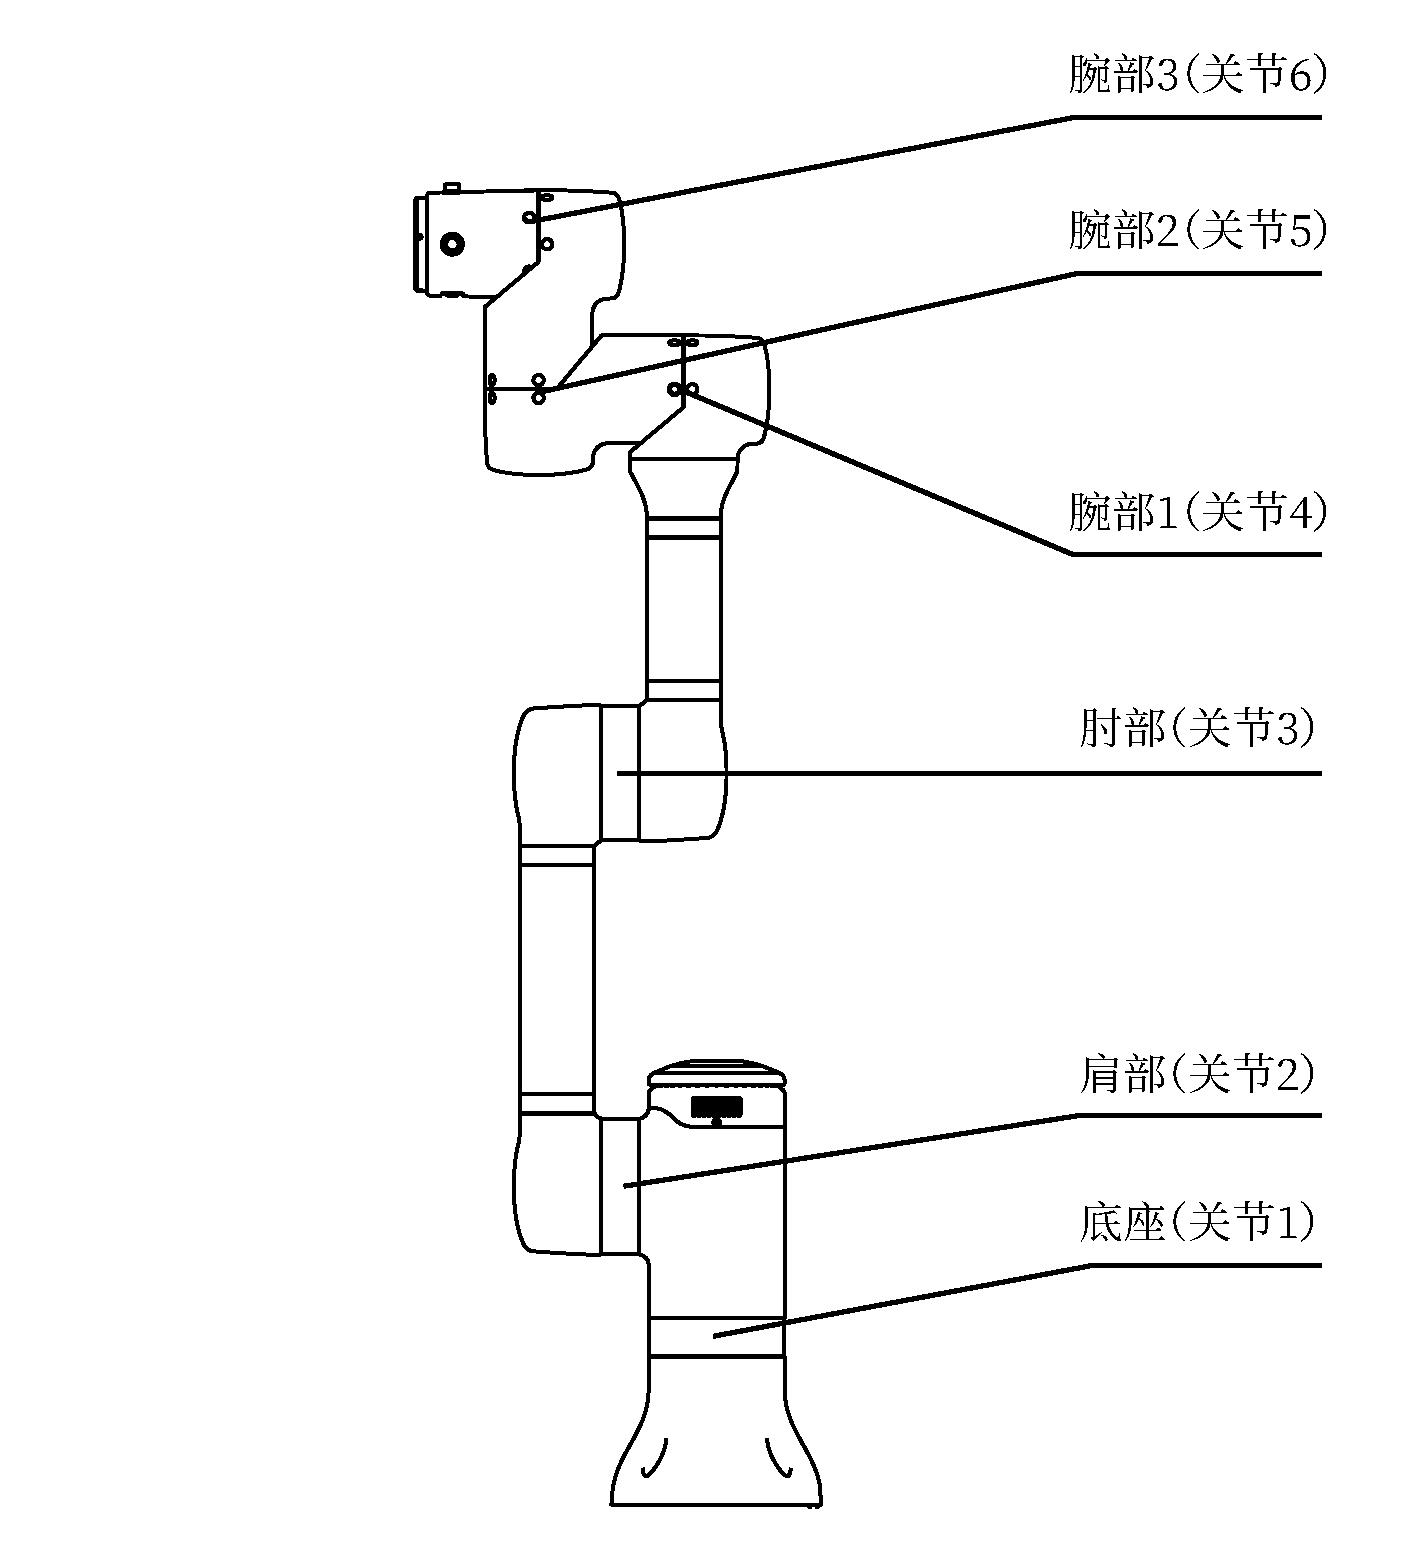
\includegraphics[height=8cm]{image/arms.pdf}
    \caption{机器人关节示意图}
    \label{fig:机器人关节示意图}
\end{figure}

机器人本体为机器人产品的执行机构,其中底座为机器人本体安装处,肩部和肘部可执行较大幅度动作,腕部1和腕部 2可执行较精细动作,腕部 3 可以连接末端工具。

控制箱为机器人系统的控制部分,可控制机器人在工作空间中的位置、姿态,连接设备的电气输入和输出端以及查看机器人的各种状态数据和信息。在实际应用场景下,为确保运行安全,通常需要在控制箱上外接急停开关(选配)。

\clearpage

如\prettyref{fig:机器人本体及控制箱连接}所示,控制箱通过机器人电缆与机器人本体连接。连接上电后\footnote{请参考\prettyref{cha:基础操作}相关内容。},用户可通过电脑、平板、手机或其他图形化终端设备的浏览器\footnote{建议使用 Google Chrome 浏览器、Microsoft Edge浏览器或其他基于Webkit 内核的现代浏览器来获得更好的体验。 }访问机器人的\LM\footnote{\LM 是本公司为机器人量身定制的机器人控制系统,所有对机器人的可视化操作和控制必须通过登录\LM 系统后再进行。}系统控制机器人。

\begin{figure}[h!]
    \centering
    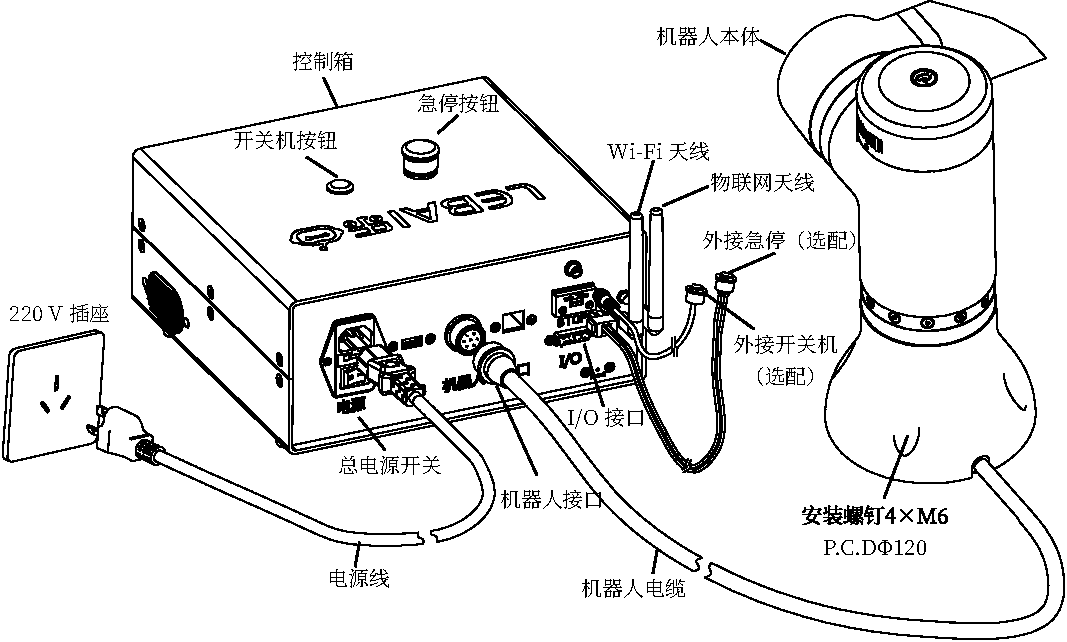
\includegraphics[width=\textwidth]{line_graphs/robot_links.pdf}
    \caption{机器人本体及控制箱连接}
    \label{fig:机器人本体及控制箱连接}
\end{figure}

\clearpage

\subsection{基础参数}

见\prettyref{tab:基础参数}。

\begin{table}[h!]
    \centering
    \rowcolors{1}{trEven}{trOdd}
    \newcommand\Thr[1]{\cellcolor{th}\sffamily\color{white}{#1}}
    \begin{tabular}{rl}
\Thr{工作半径} &		$638\mm $ \\
\Thr{有效负载   } &	$\le 3\kg$\\
\Thr{自重   } &	$9.5\kg$\\
\Thr{重复精度   } &	$\pm 0.5\mm$\\
\Thr{末端速度   } &	$\le 2\unit{m/s}$\\
\Thr{功耗   } &	典型功耗$150\unit{W}$\\
\Thr{安装方式   } &	正装、倒装、侧装\\
\Thr{安装面积   } &	$\approx 160 \unit{cm^2}$\\
\Thr{主机箱尺寸 } &	$270\times 250\times 130(H) \mm$\\
    \end{tabular}
    \caption{乐白机器人基础参数}
    \label{tab:基础参数}
\end{table}

机器人最大允许有效负载取决于重心偏移,如\prettyref{fig:有效负载图}。重心偏移定义为工具输出法兰的中心与重心之间的距离。

\begin{figure}[ht]
	\centering
	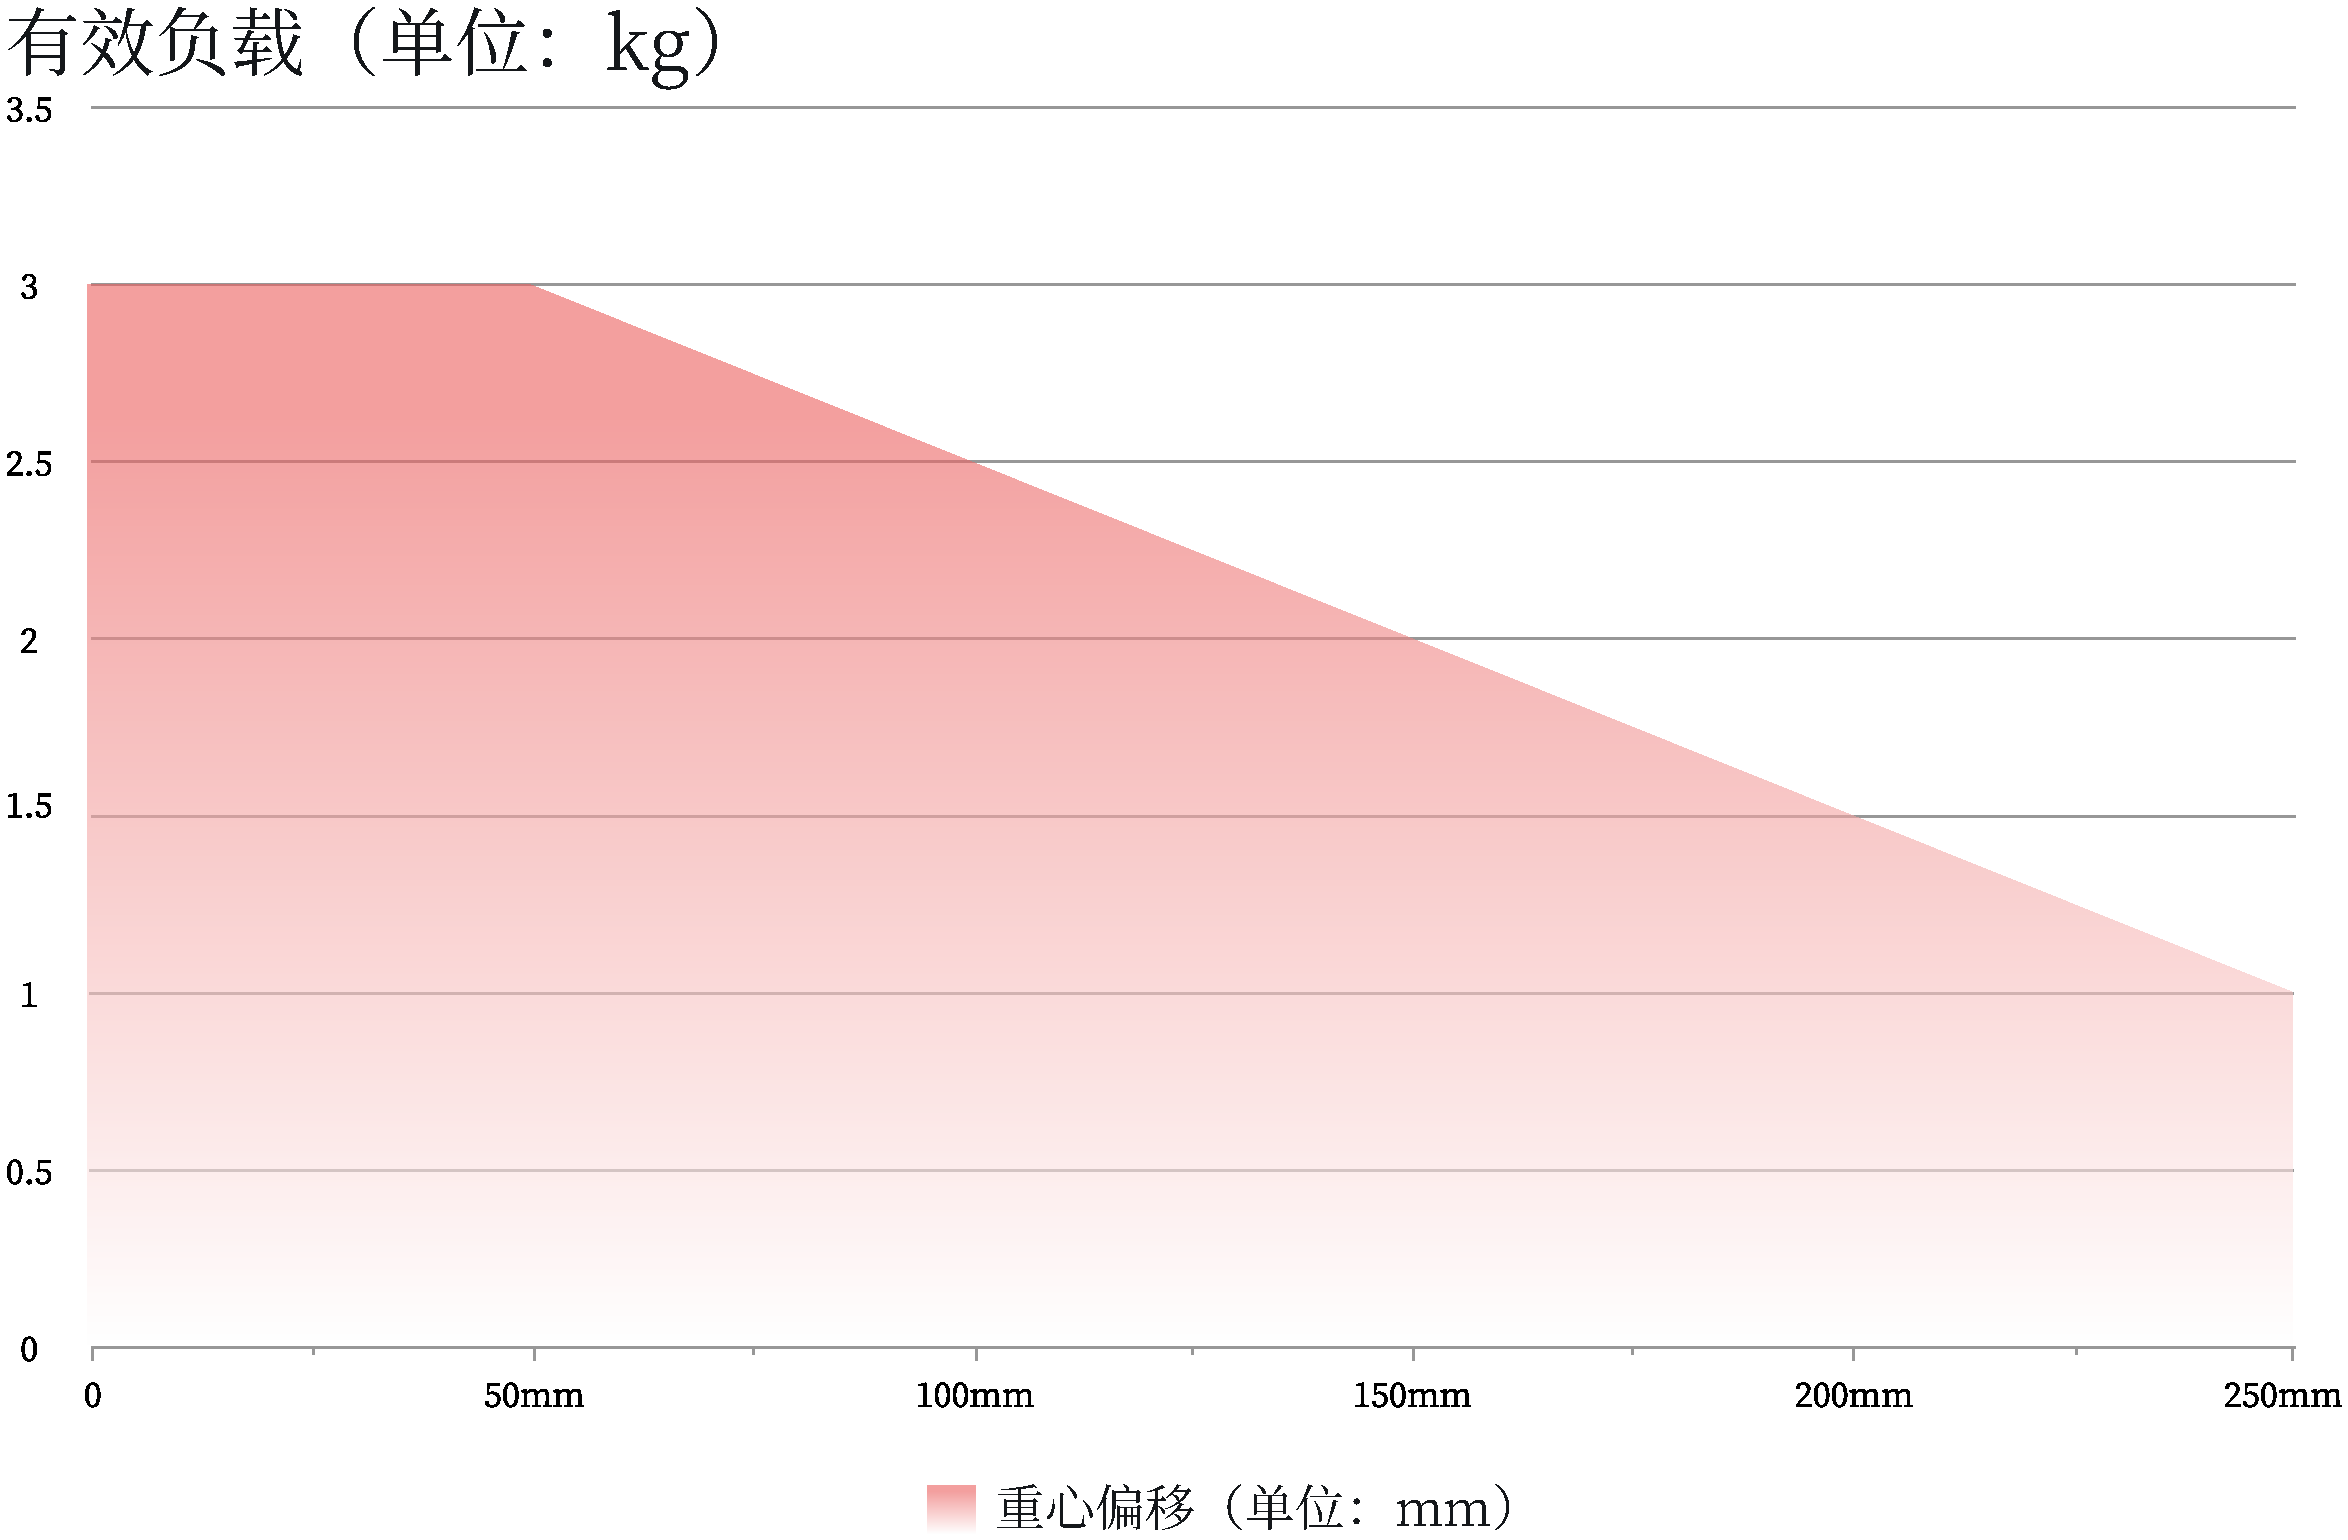
\includegraphics[width=0.8\textwidth]{line_graphs/effective_payload.pdf}
	\caption{有效负载图}
	\label{fig:有效负载图}
\end{figure}

\danger[警告]{\begin{itemize}
	\item 负载条件应在图表所示范围内;
	\item 图中显示的有效负载表示的是最大负载能力,在任何情况下,都不应该超过图中所示的最大重量;
	\item 超过允许值会导致机器内部件的提早损坏。
\end{itemize}}

\subsection{运动轴}

见\prettyref{tab:运动轴}。

\begin{table}[ht]{
    \centering
    \rowcolors{1}{trEven}{trOdd}
    \def\dps{\unit{^\circ/s}}
    \begin{tabular}{ccc}
\rowcolor{th} \Th{关节} &	\Th{运动范围} &	\Th{最大速度}\\
关节1   &	无限制  &	$180\dps$ \\
关节2   &	无限制  &	$180\dps$ \\
关节3   &	无限制  &	$180\dps$ \\
关节4   &	无限制  &	$180\dps$ \\
关节5   &	无限制  &	$180\dps$ \\
关节6   &	无限制  &	$180\dps$ \\
    \end{tabular}
    \caption{乐白机器人运动轴}
    \label{tab:运动轴}
}
    \footnotesize{注:以上所提的关节运动范围无限制需排除机器人自干涉的情况,自干涉的情况因实际运动场景而有差异}
\end{table}

\clearpage

\subsection{工作空间}

见\prettyref{fig:机器人运动范围}。

\begin{figure}[ht]
    \centering
    \subfigure[沿$Z$轴方向]{
    	\begin{minipage}[b]{0.45\textwidth}\centering
   		 	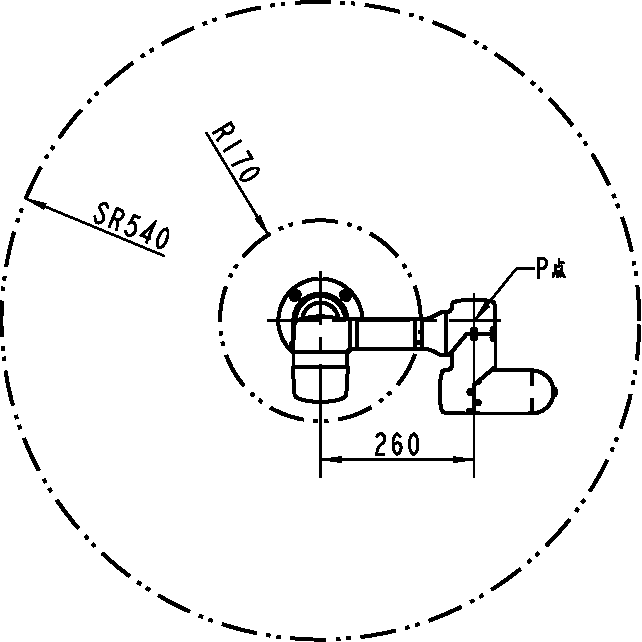
\includegraphics[width=\linewidth]{line_graphs/view-via-z.pdf}
    	\end{minipage}
    }
    \subfigure[沿$X$轴或$Y$轴方向]{
    	\begin{minipage}[b]{0.45\textwidth}\centering
   		 	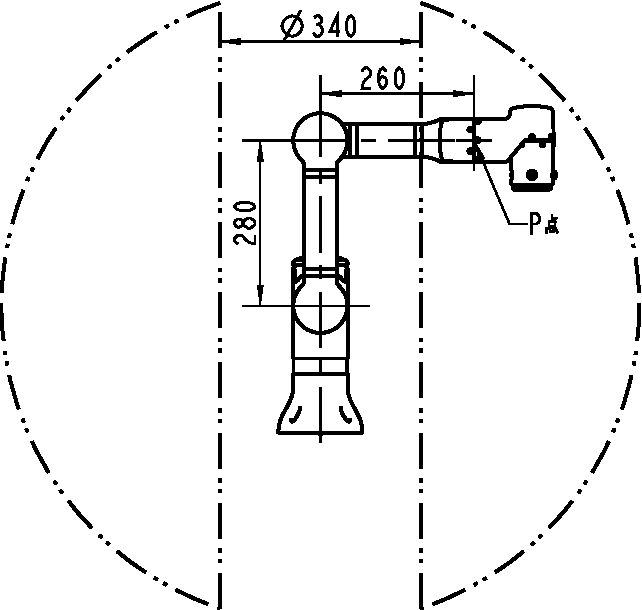
\includegraphics[width=\linewidth]{line_graphs/view-via-xy.pdf}
    	\end{minipage}
    }
    \caption{乐白机器人工作空间示意图}
    \label{fig:机器人运动范围}
\end{figure}

\clearpage

\subsection{I/O接口}

LM3提供的I/O接口有两部分:控制箱和末端法兰盘,根据不同的应用场景,您可以选择不同位置的I/O接口来实现相应的I/O操作。

\begin{enumerate}
    \item 如\prettyref{fig:控制箱IO}和\prettyref{tab:控制箱IO},机器人控制箱提供:
    \begin{itemize}
        \item 4个数字输入,4个数字输出接口;
        \item 2个模拟输入,2个模拟输出接口。
    \end{itemize}

\begin{figure}[ht]
    \centering
    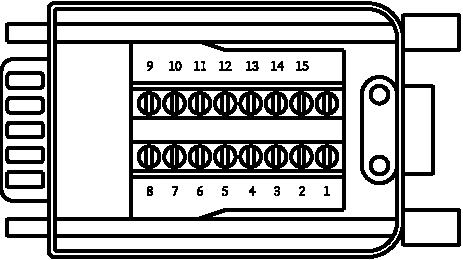
\includegraphics[height=3cm]{line_graphs/robot_box_io_plugin.pdf}
    \caption{控制箱I/O硬件接口示意图}
    \label{fig:控制箱IO}
\end{figure}

\begin{table}[ht]
    \centering\small
    % \rowcolors{1}{trEven}{trOdd}
    \def\tE{\cellcolor{trEven}}
    \def\tO{\cellcolor{trOdd}}
\begin{tabular}{cll}
\rowcolor{th} \Th{序号}	&  \Th{功能}	& \Th{性能参数}\\
\tO  1	& \tO 电源正极	& \tO $24\unit{V}$  \\
\tE  2	& \tE 模拟输出1 & \tE \\
\tO  3	& \tO 模拟输出2 & \multirow{-2}{5cm}{\tE 电压型:输出电压$0\sim 10\unit{V}$\\电流型:输出电流$4\sim 20\unit{mA}$}\\
\tE  4	& \tE 数字输出1	& \tO \\
\tO  5	& \tO 数字输出2	& \tO \\
\tE  6	& \tE 数字输出3	& \tO \\
\tO  7	& \tO 数字输出4	& \multirow{-4}{5cm}{\tO 输出电压$24\unit{V}$,最大电流$2\unit{A}$}\\
\tE  8	& \tE 电源负极	& \tE \\
\tO  9	& \tO 模拟输入1 & \tO \\
\tE  10	& \tE 模拟输入2	& \multirow{-2}{5cm}{\tO 电压型:输出电压$0\sim 10\unit{V}$\\电流型:输出电流$4\sim 20\unit{mA}$    }\\
\tO  11	& \tO 数字输入1	& \tE \\
\tE  12	& \tE 数字输入2	& \tE \\
\tO  13	& \tO 数字输入3	& \tE \\
\tE  14	& \tE 数字输入4	& \multirow{-4}{5cm}{\tE 输入电压$3\sim 30\unit{V}$}\\
\tO  15	& \tO 电源负极	& \tO \\
% \tE GND & \tE & \tE \\
\end{tabular}
\caption{控制箱I/O接口引脚说明}
\label{tab:控制箱IO}
\end{table}
% \clearpage
    \item 如\prettyref{fig:法兰盘IO}和\prettyref{tab:法兰盘IO},末端法兰盘上提供:
    \begin{itemize}
        \item 2个数字输入接口;
        \item 2个数字输出接口。
    \end{itemize}

\begin{figure}[ht]
    \centering
    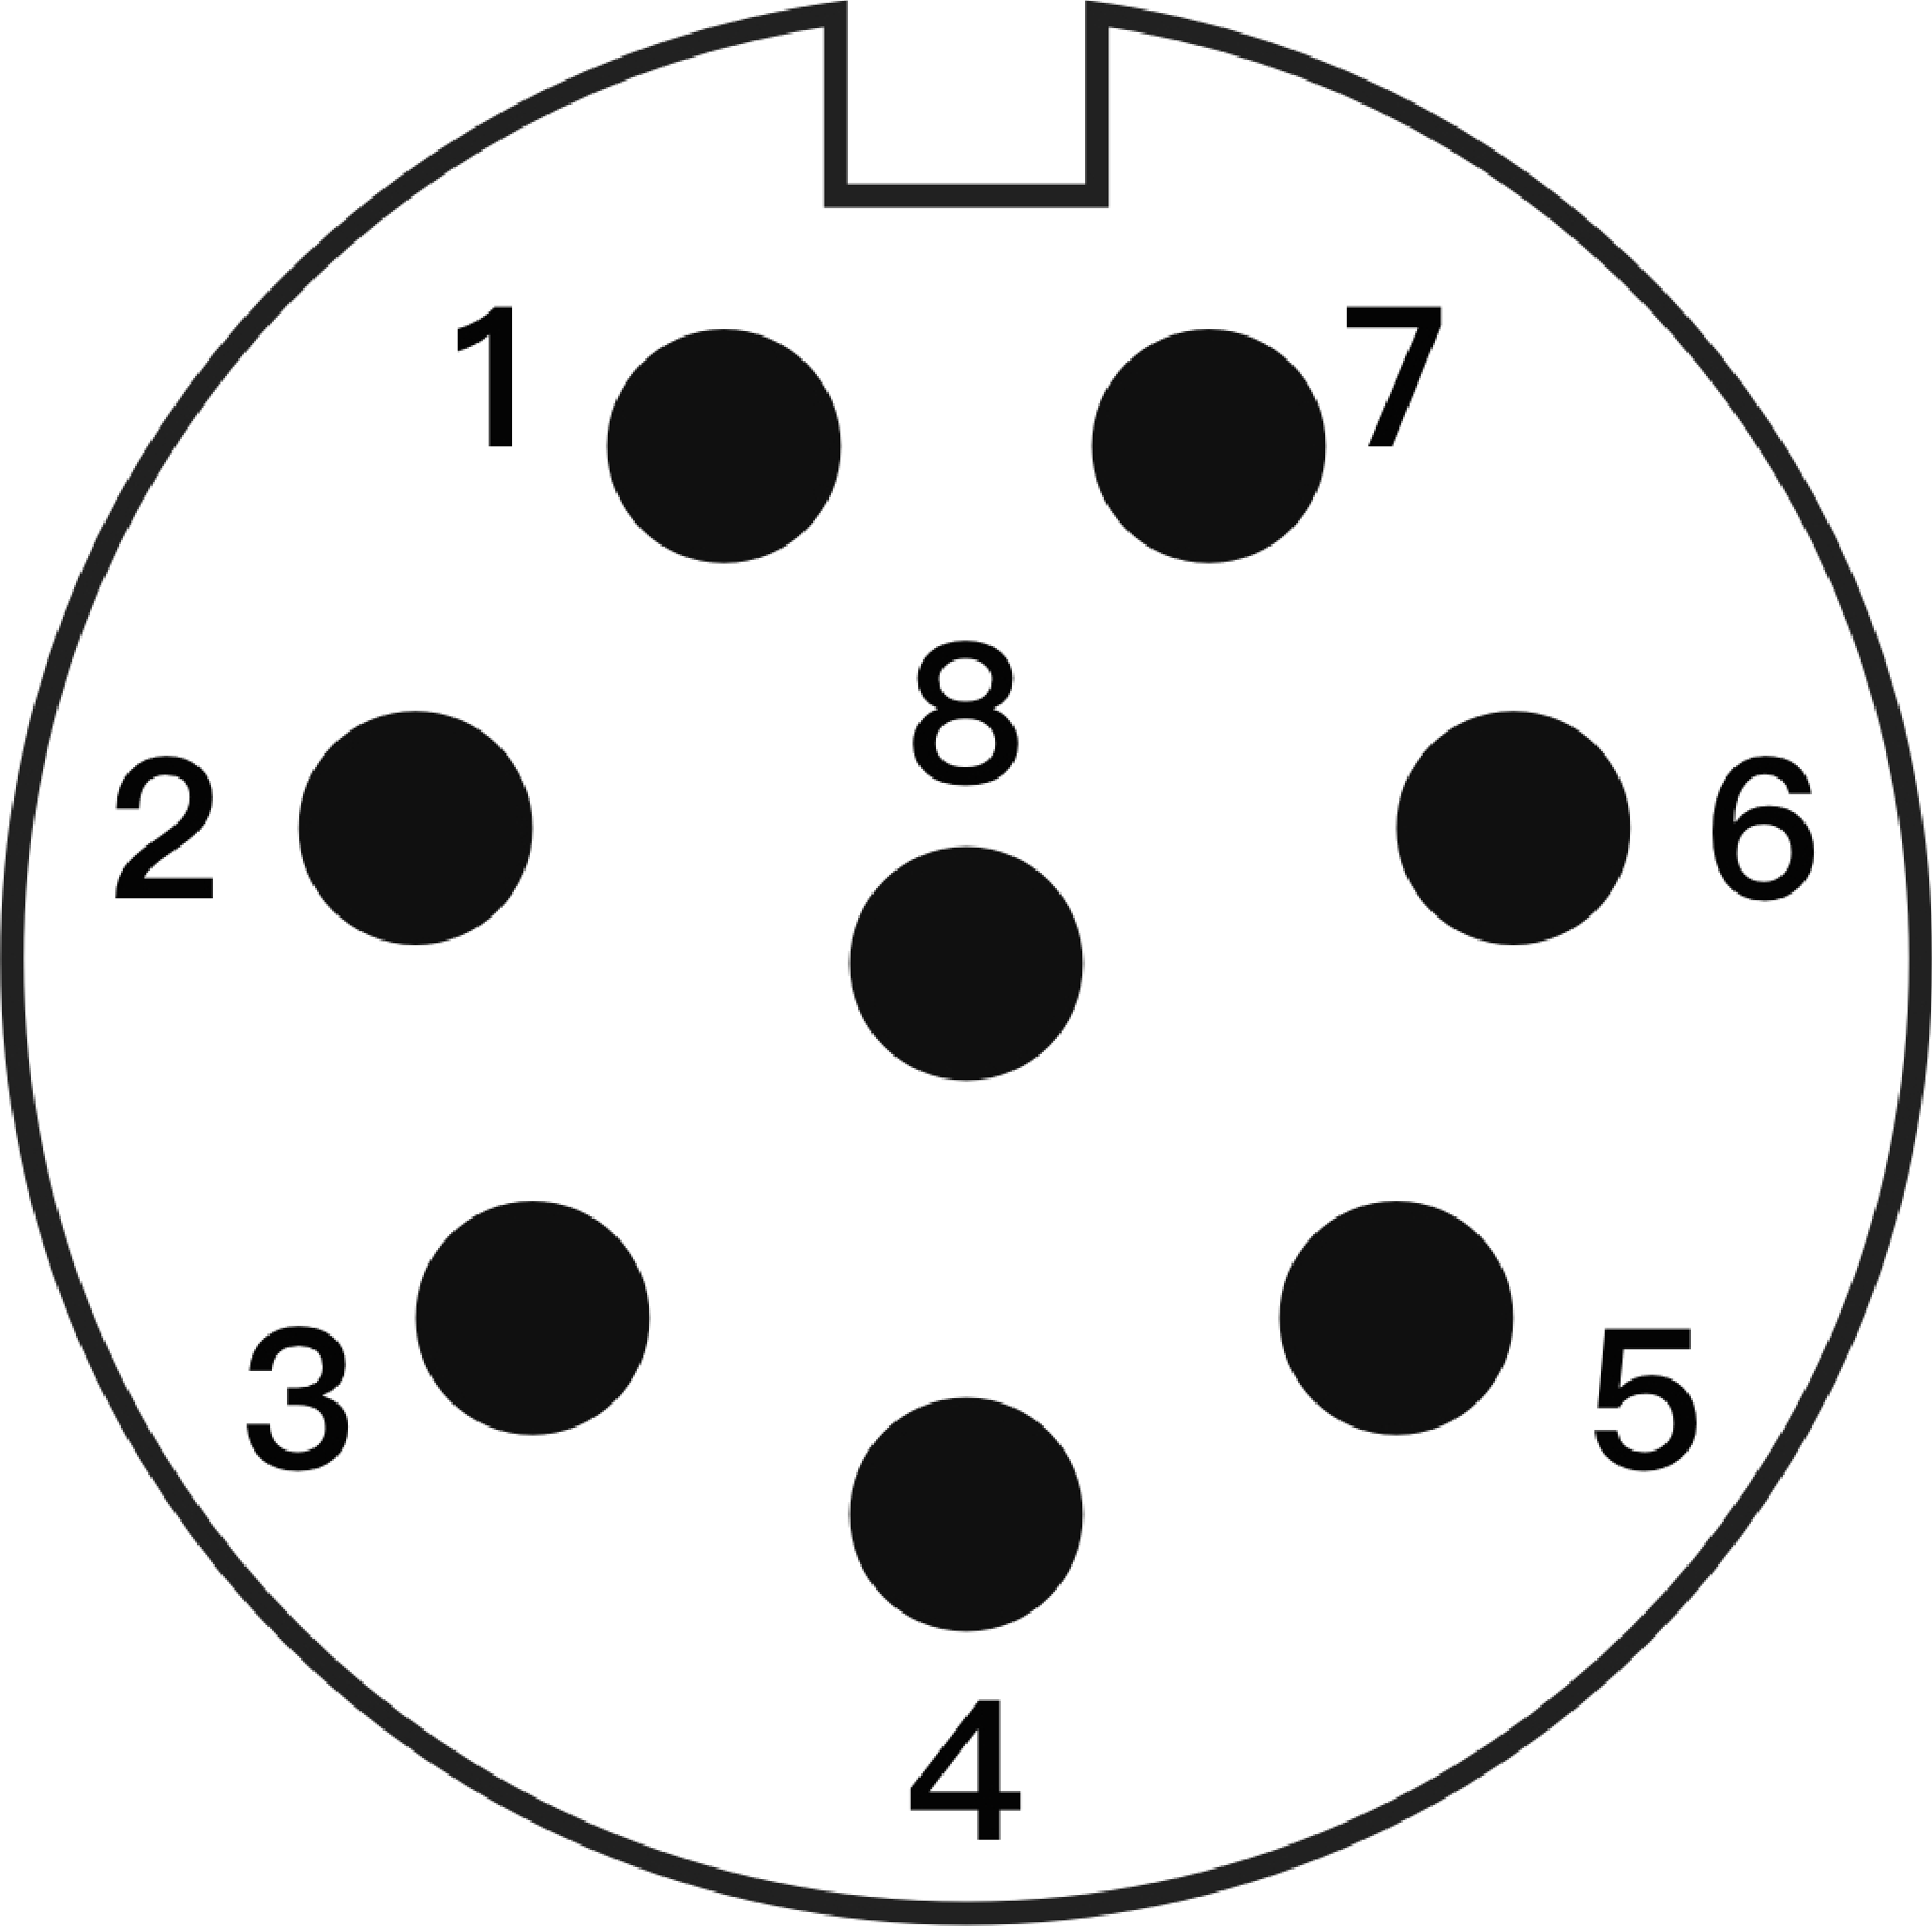
\includegraphics[height=2cm]{image/35.pdf}
    \caption{末端法兰盘 I/O硬件接口示意图}
    \label{fig:法兰盘IO}
\end{figure}

\begin{table}[ht]
    \centering\small
    \rowcolors{1}{trEven}{trOdd}
    \def\tE{\cellcolor{trEven}}
    \def\tO{\cellcolor{trOdd}}
\begin{tabular}{cll}
   \rowcolor{th}\Th{序号}	&  \Th{功能}	& \Th{性能参数}\\
    1	&   电源正极 & \tO \\
    2	&   电源负极 & \multirow{-2}{5cm}{\tO
            电压$24\unit{V}$,最大电流$2\unit{A}$    }\\
    3	&   数字输出1	&  \tE \\
    4	&   数字输出2	&   \multirow{-2}{5cm}{\tE 输出电压$24\unit{V}$,最大电流$2\unit{A}$}\\
    5	&   CANH	&  CAN通信总线高电平 \\
    6	&   CANL	& CAN通信总线低电平  \\
    7	&   数字输入1	&  \tO \\
    8	&   数字输入2	&  \multirow{-2}{5cm}{\tO
            输入电压$3\sim 30\unit{V}$
    } \\
\end{tabular}
\caption{末端法兰盘I/O引脚说明}
\label{tab:法兰盘IO}
\end{table}

\end{enumerate}

% \clearpage

\subsection{网络连接}

LM3提供以太网、Wi-Fi(2.4 GHz) 热点网络、4G物联网三种网络连接方式。其中:以太网和Wi-Fi网络连接用于提供给用户操作和连接机器人使用,4G物联网连接目前仅用于设备基础信息\footnote{设备基础信息仅限于:设备名称,设备网络连接类型及状态,软件系统版本,系统运行错误信息且不包含任何客户业务数据(包括且不限于场景数据等)。如需其他信息的上报,乐白将事前获得您的授权同意后才进行。}的数据上报。

% \vfill

\clearpage

\section{机器人安装}

如\prettyref{fig:机器人安装方式},LM3机器人支持三种安装方式:正装、倒装、侧装(侧装时注意机器人电缆出口必须朝下)。

\begin{figure}[ht]
    \centering
    \subfigure[正装]{
		\begin{minipage}[b]{0.3\textwidth}\centering
			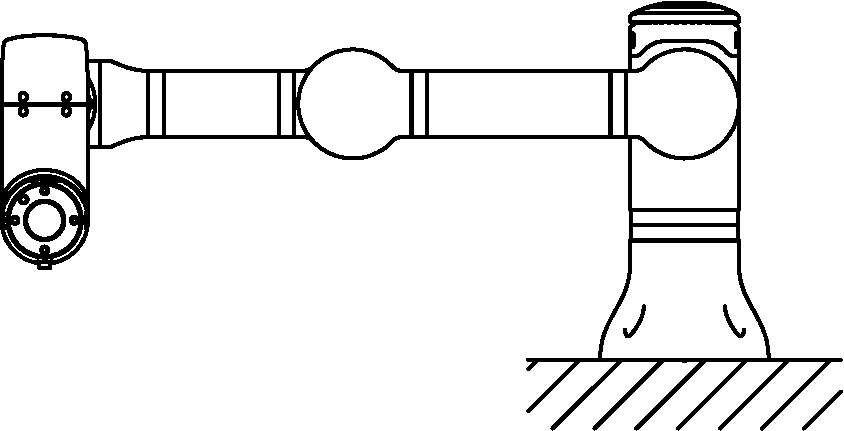
\includegraphics[width=\linewidth]{line_graphs/install_direction_up.pdf}
		\end{minipage}
	}
    \subfigure[倒装]{
    	\begin{minipage}[b]{0.3\textwidth}\centering
   		 	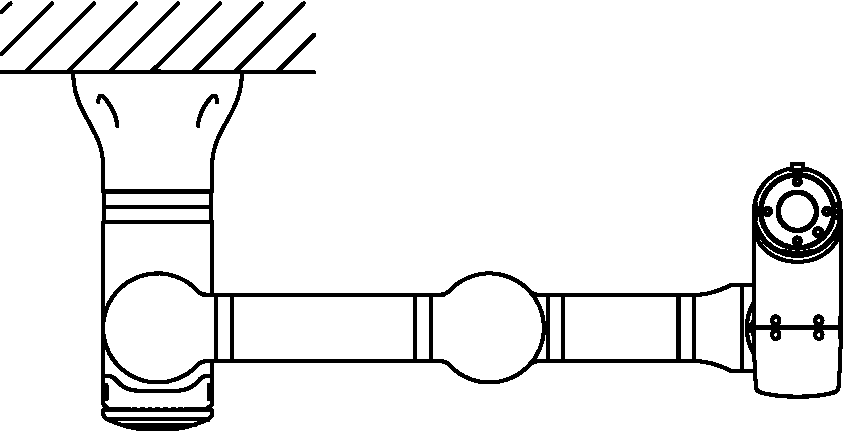
\includegraphics[width=\linewidth]{line_graphs/install_direction_down.pdf}
    	\end{minipage}
    }
    \subfigure[侧装]{
    	\begin{minipage}[b]{0.3\textwidth}\centering
   		 	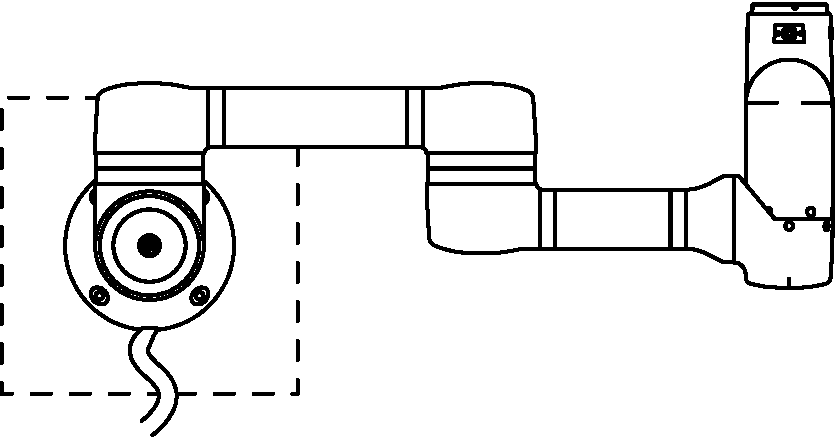
\includegraphics[width=\linewidth]{line_graphs/install_direction_side.pdf}
    	\end{minipage}
    }
    \caption{机器人安装方式}
    \label{fig:机器人安装方式}
\end{figure}

% \clearpage

\begin{figure}[ht]
    \centering
    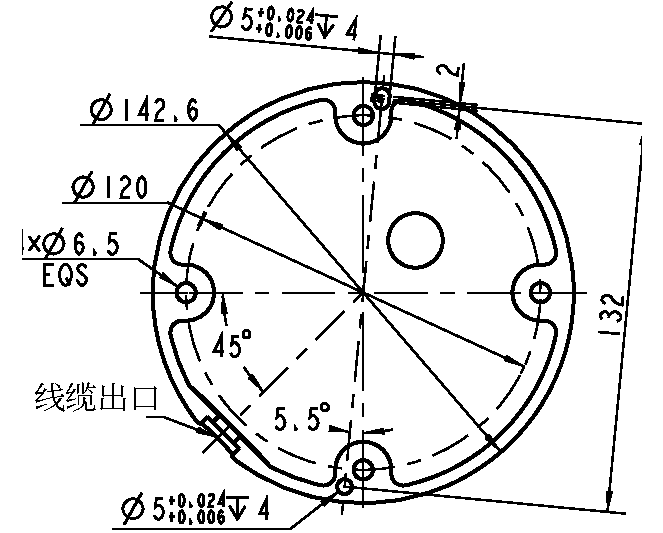
\includegraphics[height=5cm]{line_graphs/bottom_surface.pdf}
    \caption{机器人底座视图}
    \label{fig:机器人底座视图}
\end{figure}

使用机器人配件包中的 4 颗 M6 螺钉,对应机器人底座(如\prettyref{fig:机器人底座视图})上的 4 个安装孔进行安装操作,建议以 $9\Nm$ 扭矩紧固这些螺钉。如果需要更准确地调整机器人位置,还可钻2 个直径$5 \mm$的孔,并用销加以固定。

\info{\begin{itemize}
\item 机器人每一个安装孔位都应固定螺钉,固定后的每个螺钉都应能提供最小抗倾覆力;
\item 机器人安装时,应扶住机器人直至底座所有螺钉全部紧固好。
\end{itemize}}

\danger[警告]{切勿将机器人(含控制箱)固定在不稳固的位置,否则可能会跌落损坏。}
